\documentclass{beamer}

\usepackage[utf8]{inputenc}
\usepackage[spanish,activeacute]{babel}
\usepackage{listings} % Trozos de código
\usepackage{graphicx} % Imágenes
\usepackage{fancyhdr} % Cabeceras
\usepackage{listings}

\usetheme{Darmstadt}
\usefonttheme{structuresmallcapsserif} 


\title{Desarrollo de un Pong en C con SDL}
\author{David Saltares Márquez \and Alberto Cejas Sánchez}


\AtBeginSection[]
{
  \begin{frame}<beamer>
    \frametitle{Índice}
    \tableofcontents[currentsection,currentsubsection]
  \end{frame}

}

\begin{document}

\begin{frame}
	\titlepage
	
    \begin{picture}(0,0)
        \put(10,-5){
\includegraphics[scale=0.1]{img/advuca.png}}
    \end{picture}
    
    \begin{picture}(0,0)
        \put(230,-15){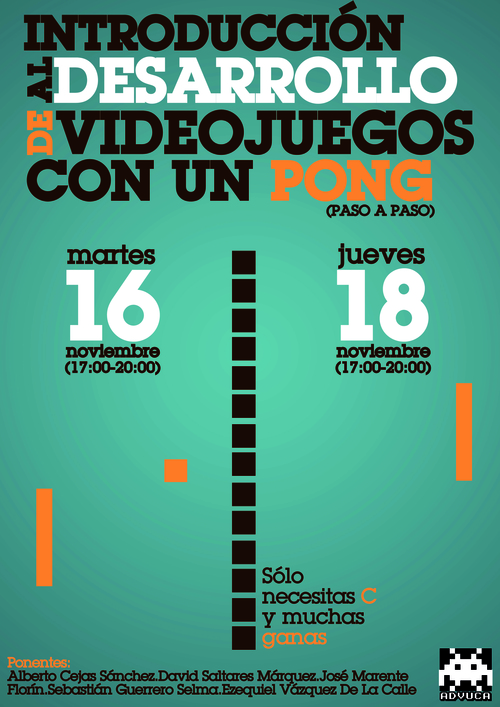
\includegraphics[scale=0.5]{img/cartel.jpg}}
    \end{picture}
    
    \begin{center}
        
\includegraphics[scale=1]{img/cc.png}
    \end{center}    
\end{frame}

\begin{frame}
	\frametitle{Índice de contenidos}
	\tableofcontents
\end{frame}


%	======= ADVUCA =======

\section{ADVUCA}

\begin{frame}
    \frametitle{¿Pero qué es la ADVUCA?}
    
    \begin{center}
        \begin{alertblock}{¡Es un acrónimo!}
            \emph{ADVUCA} $\rightarrow$ Asociación de Desarrollo de Videojuegos de la UCA
        \end{alertblock}        
    \end{center}
    
    \begin{columns}[c]
		\column{150pt}
		\begin{block}{La fundamos}
            \begin{itemize}
                \item David Saltares Márquez
                \item Jose Marente Florín
                \item Alberto Cejas Sánchez
                \item Francisco Javier Santacruz López-Cepero
                \item Sebastián Guerrero Selma
            \end{itemize}            
        \end{block}
	\begin{center}
	    Somos alumnos de la ESI
	\end{center}
		\column{150pt}
		\begin{center}
			
\includegraphics[scale=0.2]{img/advuca.png}
		\end{center}
	\end{columns} 
\end{frame}

	
\begin{frame}
	\frametitle{Nuestros objetivos}
	
	\begin{columns}[c]
		\column{75pt}
		\begin{center}
			
\includegraphics[scale=0.3]{img/link.png}
		\end{center}
		\column{225pt}
		
		\begin{center}
			Este taller es sólo el principio
		\end{center}		
		
		\begin{block}{Pretendemos}
            \begin{itemize}
                \item Formar grupos de desarrollo de videojuegos
				\item Ofrecer documentación sobre creación de videojuegos
				\item Colaborar con asignaturas de la carrera
				\item Trabajo con grupos interdisciplinares (programación, grafismo, sonido...)
				\item ¡Divertirnos!
            \end{itemize}            
        \end{block}        
	\end{columns}
\end{frame}

\begin{frame}
	\frametitle{Inscríbete}
	
	\begin{columns}[c]
		\column{150pt}
	
	http://blog.advuca.com
		
	\begin{block}{Sólo necesitas}
            \begin{itemize}
                \item Matrícula de la UCA
		\item Datos personales
		\item No pedimos pasta, sólo ganas de aprender ;-)
            \end{itemize}            
        \end{block}        
		\column{150pt}
		\begin{center}
			
\includegraphics[scale=0.22]{img/iwantyou.jpg}
		\end{center}
	\end{columns} 
	
\end{frame}


%	======= DISEÑO DE VIDEOJUEGOS =======

\section{Videojuegos}
\begin{frame}
	\frametitle{El equipo}
	
	Puede que tus primeros juegos los desarrolles de forma individual,
	pero los equipos suelen componerse de:
		
	\begin{columns}[c]
	\column{200pt}	
	
	\begin{block}{Componentes de un equipo}
		\begin{itemize}
			\item Diseñadores
			\item Ingenieros y programadores
			\item Artistas 2D
			\item Artistas 3D
			\item Sonido
			\item Otro equipo: soporte, marketing etc.
		\end{itemize}            
	\end{block}
	
	\column{100pt}
	\begin{center}
	    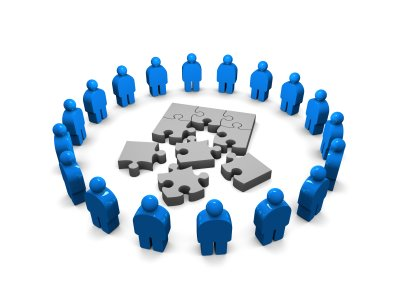
\includegraphics[scale=0.3]{img/collaborate.jpg}
	\end{center}
	
	
	\end{columns}
\end{frame}

\begin{frame}
	\frametitle{El proceso}
	
	Aunque te de una pereza tremenda deberías mantener una mínima
	disciplina o tu proyecto se quedará en una ¿buena? idea.
		
	\begin{block}{Pasos}
		\begin{itemize}
			\item Definir el juego (tipo, jugabilidad, personajes...)
			\item Ingeniería del Software (¿acaso creías que no valía para nada?)
			\begin{itemize}
			    \item Lo más importante es planificarse bien
			\end{itemize}
			\item Implementación
			\item Documentación (¡no lo dejes para el final!)
			\begin{itemize}
			    \item Hay técnicas de documentación automática fáciles y productivas
			\end{itemize}
			\item Muchas pruebas
			\item Lanzamiento
		\end{itemize}            
	\end{block}        
	
\end{frame}

\begin{frame}
	\frametitle{¡Importante!}
	
	\begin{center}
		Recuerda, no creas que tu primeros proyectos serán algo así:
	\end{center}	
	
	\begin{center}
		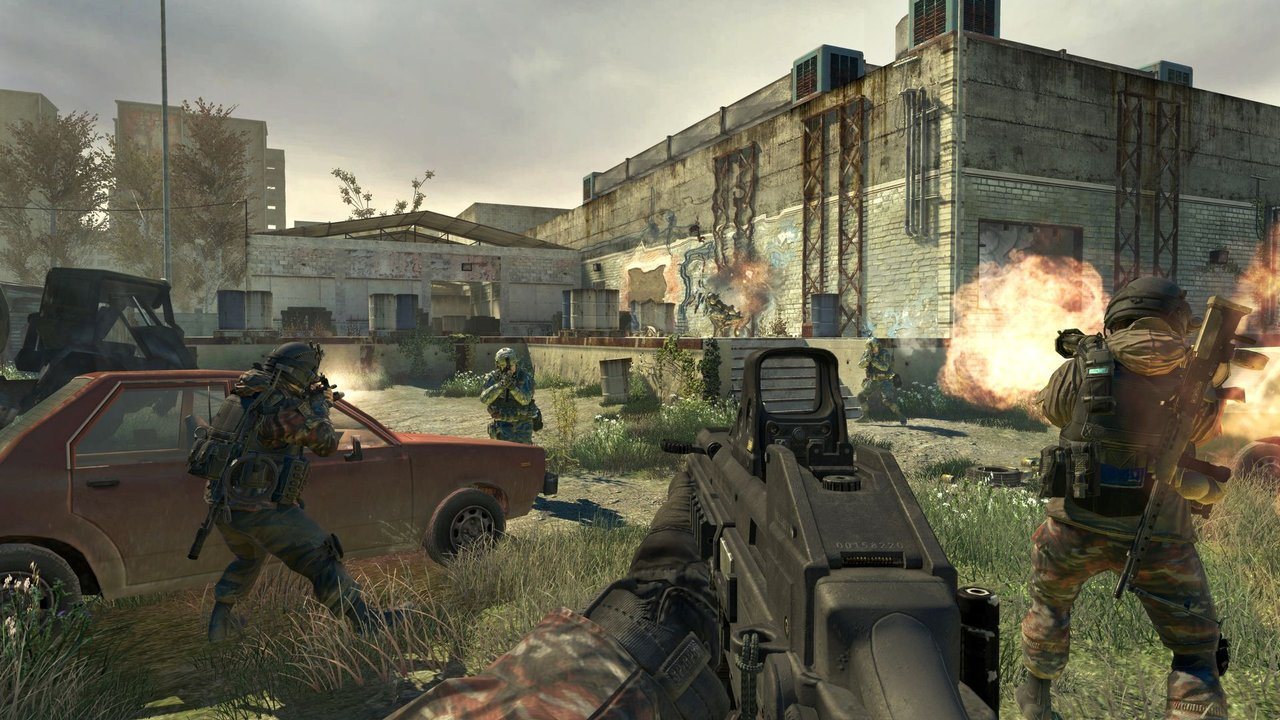
\includegraphics[scale=0.2]{img/codmw2.jpg}
	\end{center}
	
	\begin{center}
		Serán como los que hacemos en clase...
	\end{center}	
\end{frame}


\begin{frame}
	\frametitle{Probablemente sean así}

	\begin{center}
	Robinson 2.0
	
	    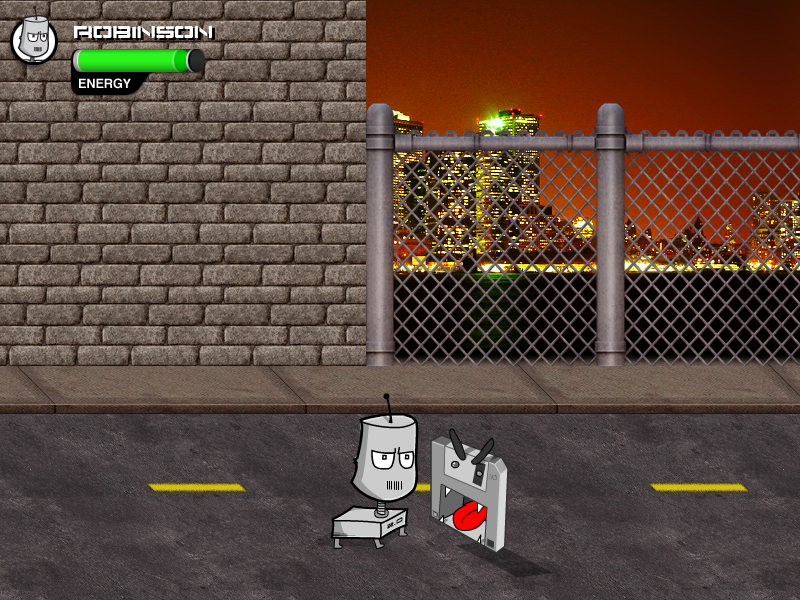
\includegraphics[scale=0.3]{img/robinson.png}
	\end{center}
\end{frame}

\begin{frame}
	\frametitle{Probablemente sean así}

	\begin{center}
	Space Penguin
	
	    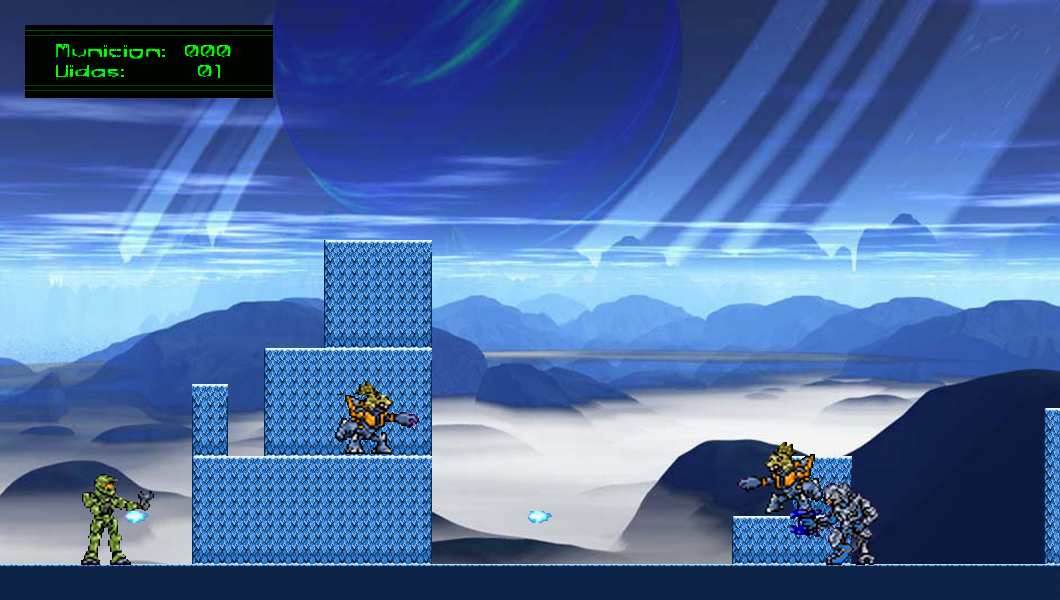
\includegraphics[scale=0.3]{img/spacepenguin.png}
	\end{center}
\end{frame}

\begin{frame}
	\frametitle{Probablemente sean así}

	\begin{center}
	Granny's Bloodbath
	
	    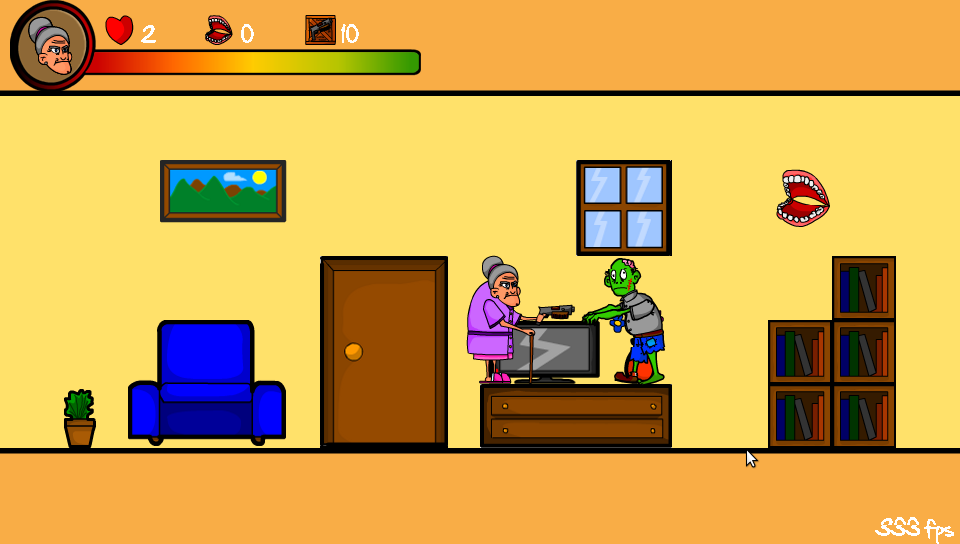
\includegraphics[scale=0.3]{img/grannysbloodbath.png}
	\end{center}
\end{frame}

\begin{frame}
	\frametitle{Probablemente sean así}

	\begin{center}
	Magic Duel
	
	    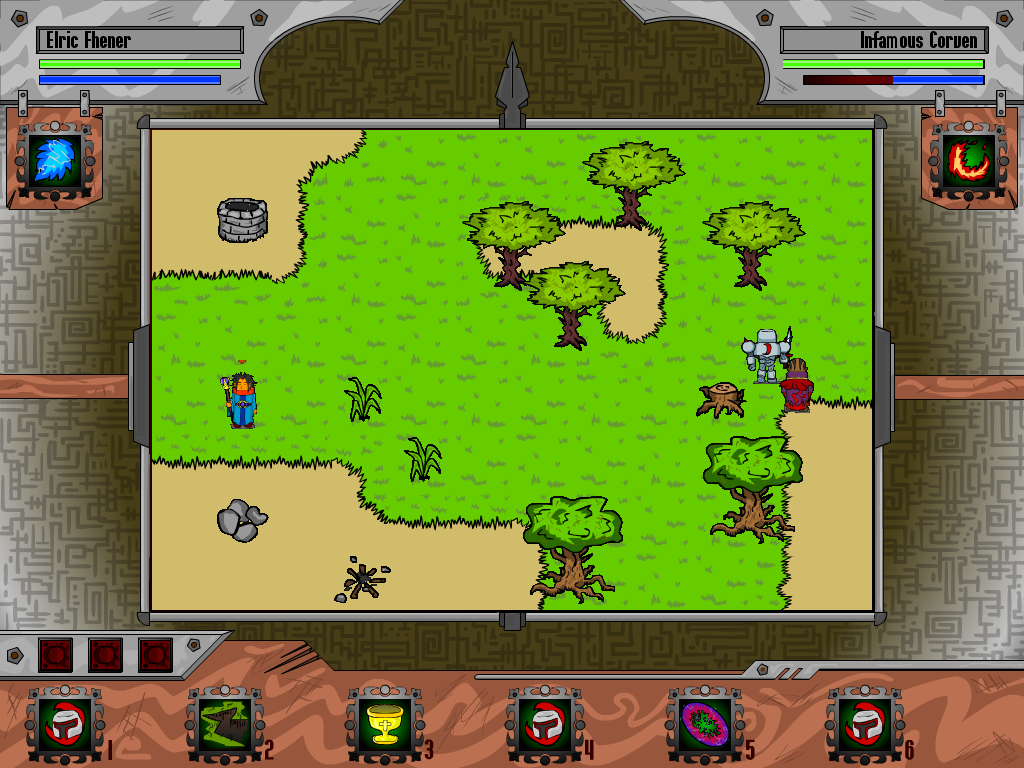
\includegraphics[scale=0.22]{img/magicduel.png}
	\end{center}
\end{frame}

\begin{frame}
	\frametitle{Diseño}
	
	\begin{center}
		Antes de lanzarse a programar hay que diseñar el juego
	\end{center}	
	
	\begin{columns}
	
	\column{175pt}
	\begin{block}{Modelado del mundo}
		\begin{itemize}
			\item Planteamiento y concepto
			\item Género
			\item Mecánicas
			\item Estructura de los niveles
			\item Personajes, enemigos y objetos
			\item Público objetivo
		\end{itemize}            
	\end{block}
	
	
	\column{125pt}
	\begin{center}
		
\includegraphics[scale=0.2]{img/assassins.jpg}
	\end{center}	
	
	
	\end{columns}
\end{frame}


\begin{frame}
	\frametitle{Game Loop}
	
	\begin{center}
		Todos los juegos siguen esta estructura, \textbf{\emph{Game Loop}}:
	\end{center}	
	
	\begin{columns}
	
	\column{150pt}
	\begin{center}
		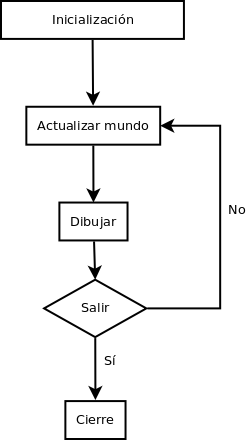
\includegraphics[scale=0.25]{img/gameloop.png}
	\end{center}	
	
	\column{150pt}
	\begin{alertblock}{Frames y movimiento}
		\begin{itemize}
			\item \emph{Actualizar}: los elementos reaccionan a su entorno y al usuario.
			\item \emph{Dibujar}: la escena se dibuja en pantalla.
			\item Si cada segundo se producen 25 iteraciones (25fps), tendremos sensación de movimiento.
		\end{itemize}            
	\end{alertblock}
	
	\end{columns}
\end{frame}

\begin{frame}
	\frametitle{Game Loop - Inicialización}
	
	Durante la etapa de inicialización se llevan a cabo las siguientes
	tareas:
	
	\begin{columns}[c]
	\column{200pt}
		
	\begin{block}{Pasos}
		\begin{itemize}
			\item Inicializar el motor y las librerías que usemos
			\item Cargar ficheros de configuración
			\item Dejar todo listo para empezar a trabajar
		\end{itemize}            
	\end{block}
	
	\column{100pt}
	
	\begin{center}
		
\includegraphics[scale=0.25]{img/engine.png}
	\end{center}	
	
	\end{columns}
	
\end{frame}

\begin{frame}
	\frametitle{Game Loop - Actualizar}
	
	Cada vez que actualizamos tenemos en cuenta:
	
	\begin{columns}[c]
	\column{175pt}
		
	\begin{block}{Actualizar}
		\begin{itemize}
			\item Entrada del usuario
			\item Red
			\item Movimiento y acciones del/los personaje/s
			\item Movimiento y acciones del/los enemigo/s, Inteligencia Artificial
			\item Colisiones, física
			\item Eventos aleatorios o asíncronos
		\end{itemize}            
	\end{block}
	
	\column{125pt}
	
	\begin{center}
		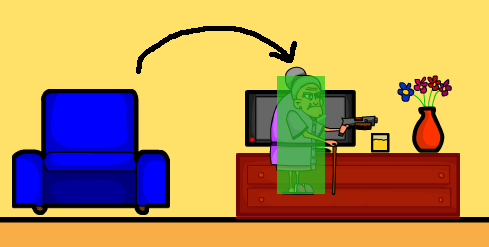
\includegraphics[scale=0.25]{img/grannycolision.png}
	\end{center}	
	
	\end{columns}
	
\end{frame}

\begin{frame}
	\frametitle{Game Loop - Dibujar}
	
	La fase de dibujado en un juego 2D:
	
	\begin{columns}[c]
	\column{175pt}
		
	\begin{block}{Dibujar}
		\begin{itemize}
			\item Dibujamos por capas, como The Gimp o Photoshop
			\item Componemos la escena por piezas
			\item Suele hacerse en orden (lejano-cercano)
			\item Algunas librerías permiten z-order
		\end{itemize}            
	\end{block}
	
	\column{125pt}
	
	\begin{center}
		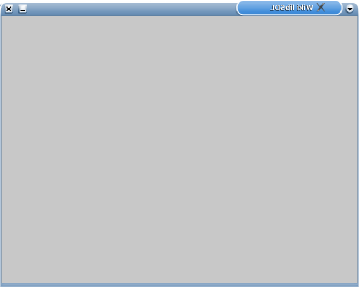
\includegraphics[scale=0.4]{img/pantalla.png}
		
		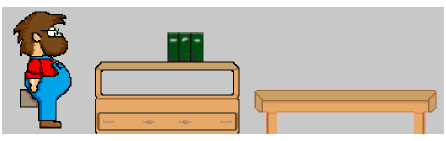
\includegraphics[scale=0.4]{img/elementos.png}
		
		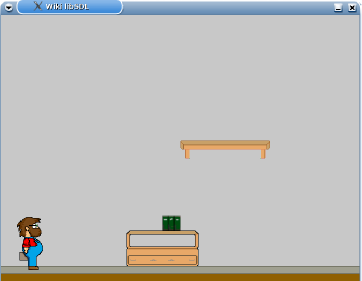
\includegraphics[scale=0.4]{img/composicion.png}
	\end{center}	
	
	\end{columns}
	
\end{frame}

\begin{frame}
	\frametitle{Game Loop - Cierre}
	
	¡Hay que recoger antes de salir!
	
	\begin{columns}[c]
	\column{175pt}
		
	\begin{block}{Cierre}
		\begin{itemize}
			\item Destruir todos los elementos del juego
			\item Cerrar las librerías en uso
		\end{itemize}            
	\end{block}
	
	\column{125pt}
	
	\begin{center}
		
\includegraphics[scale=0.25]{img/tidy.jpg}
	\end{center}	
	
	\end{columns}
	
	\begin{center}
	    ¡Los descuidos de memoria son muy peligrosos!
	\end{center}
	
\end{frame}


\section{Pong}
\begin{frame}
	\frametitle{Pong original}
	
    \begin{center}
        \textbf{La leyenda}
    \end{center}
	
    \begin{center}
		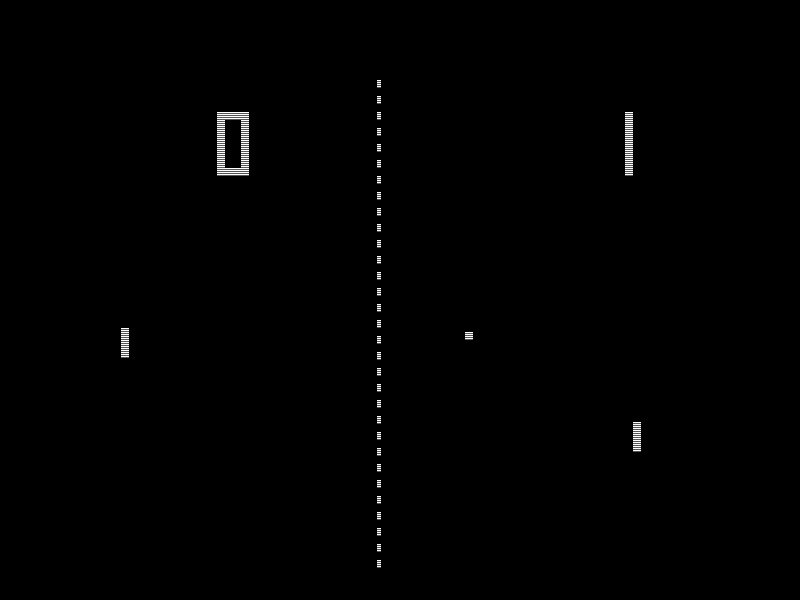
\includegraphics[scale=0.4]{img/pong-original.png}
	\end{center}	

\end{frame}

\begin{frame}
	\frametitle{Pong original}
	
	Para ir abriendo boca:
	
	\begin{columns}[c]
	\column{175pt}
		
	\begin{block}{Pong Facts}
		\begin{itemize}
            \item Uno de los primeros videojuegos de la historia.
			\item Creado por Nolan Bushnell en 1972 para Atari.
            \item Atari demandó a muchísimas copias de Pong.
            \item Tuvo un grandioso éxito... y ahora estamos aquí.
		\end{itemize}            
	\end{block}
	
	\column{125pt}
	
	\begin{center}
		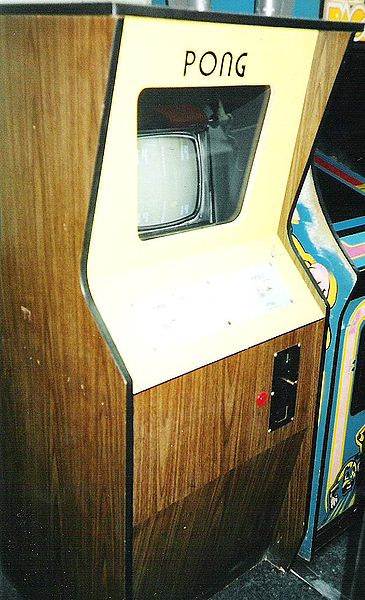
\includegraphics[scale=0.3]{img/pong-recreativa.jpg}
	\end{center}	
	
	\end{columns}
	
\end{frame}

\begin{frame}
	\frametitle{Pong - Diseño}
	
	\begin{center}
	Toca diseñar nuestro Pong, ¡manos a la obra!
	\end{center}
	
	\begin{columns}[c]
	\column{175pt}
		
	Recordad	
	
	\begin{block}{Previously...}
		\begin{itemize}
			\item Planteamiento, concepto y género
			\item Personajes, enemigos y objetos
			\item Mecánicas
		\end{itemize}            
	\end{block}
	
	\column{125pt}
	
	\begin{center}
		
\includegraphics[scale=0.3]{img/Lamp-256.png}
	\end{center}	
	
	\end{columns}
	
	\begin{center}
	Con más más formalidad en el Game Design Document
	\end{center}
	
\end{frame}

\begin{frame}
	\frametitle{Pong - Diseño - Planteamiento}
	
	\begin{columns}[c]
	\column{175pt}	
	
	\begin{block}{Planteamiento}
		\begin{itemize}
			\item Juego arcade
			\item Simulación muy básica del tenis
			\item Jugador VS IA
		\end{itemize}            
	\end{block}
	
	\column{125pt}
	
	\begin{center}
		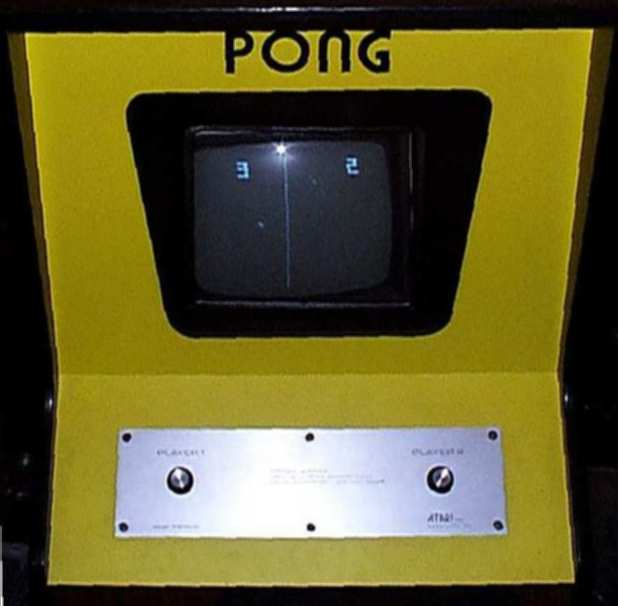
\includegraphics[scale=0.2]{img/pong-recreativa-2.jpg}
	\end{center}
	
	\begin{center}
	    Esta recreativa derrocha amor
	\end{center}	
	
	
	\end{columns}
	
\end{frame}

\begin{frame}
	\frametitle{Pong - Diseño - Mecánica}
	
	\begin{columns}[c]
	\column{175pt}	
	
	\begin{block}{Palas}
		\begin{itemize}
			\item Tablero rectangular
			\item El jugador controla una pala
			\item La IA controla otra pala
			\item Deben golpear una pelota para marcar en el campo contrario
			\item La IA será invencible
			\item El jugador debe aguantar lo máximo posible
			\item Superación del récord
		\end{itemize}            
	\end{block}
	
	\column{125pt}
	
	\begin{center}
		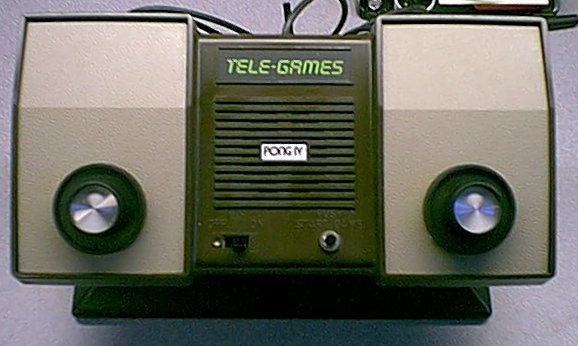
\includegraphics[scale=0.45]{img/telepong.jpg}
	\end{center}
	
	\begin{center}
	    Dos jugadores en el mismo pad
	\end{center}	
	
	\end{columns}
	
\end{frame}

\begin{frame}
	\frametitle{Pong - Diseño - Jugador}
	
	\begin{columns}[c]
	\column{175pt}	
	
	\begin{block}{Jugador humano}
		\begin{itemize}
			\item Movimiento: arriba y abajo
			\item Sin salirse del tablero
		\end{itemize}            
	\end{block}
	
	\column{125pt}
	
	\begin{center}
		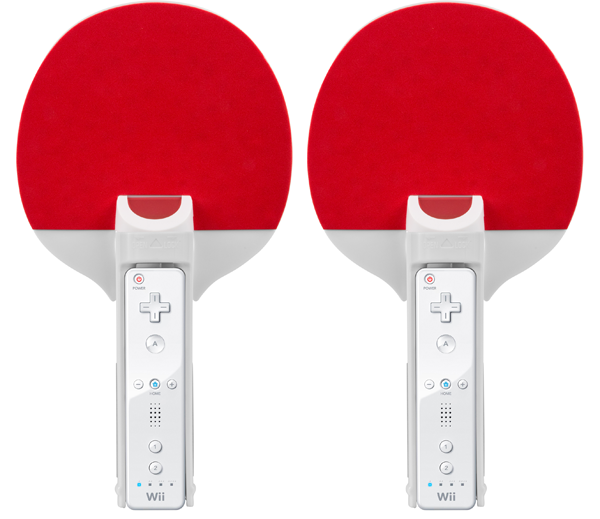
\includegraphics[scale=0.6]{img/wiipong.png}
	\end{center}	
	
	\begin{center}
	Estas \textbf{NO} serán nuestras palas
	\end{center}
	
	\end{columns}
	
\end{frame}

\begin{frame}
	\frametitle{Pong - Diseño - Bola}
	
	\begin{columns}[c]
	\column{175pt}	
	
	\begin{block}{Bola}
		\begin{itemize}
			\item Movimiento rectilíneo uniforme
			\item Rebotes en palas y bordes
			\item No tendremos en cuenta ángulos de choque
		\end{itemize}            
	\end{block}
	
	\column{125pt}
	
	\begin{center}
		
\includegraphics[scale=0.4]{img/pelota.png}
	\end{center}	
	
	\begin{center}
	    Aún no tendremos que desempolvar los libros de física de la ESO
	\end{center}
	
	\end{columns}
	
\end{frame}



\section{SDL}
\begin{frame}
    \frametitle{SD... ¿qué?}
    
    
    \begin{columns}[c]
		\column{220pt}
		\begin{block}{¿Qué es la SDL?}
            \begin{itemize}
                \item Librería multimedia para aplicaciones 2D
                \item Escrita en lenguaje C
                \item Compatible con multitud de lenguajes (C, C++, Python...)
                \item Multiplataforma (Linux, Windows, Mac, PSP...)
                \item Completamente libre (LGPL)
            \end{itemize}            
        \end{block}
        
        \begin{center}
        Es extensible mediante complementos
        \end{center}
        
		\column{100pt}
		\begin{center}
			
\includegraphics[scale=0.2]{img/sdl.jpeg}
		\end{center}
	\end{columns} 
\end{frame}

\begin{frame}
    \frametitle{Características}
    
    
    \begin{columns}[c]
		\column{160pt}
		\begin{block}{Lo que SÍ ofrece SDL}
            \begin{itemize}
                \item Vídeo
                \item Entrada
                \item Sonido
                \item Red
                \item Fuentes
                \item CD-ROM
                \item Control de tiempo
            \end{itemize}            
        \end{block}
        
		\column{160pt}
        
        \begin{alertblock}{Lo que NO ofrece SDL}
            \begin{itemize}
                \item Física
                \item Colisiones
                \item Inteligencia Artificial
                \item Gestión de recursos
                \item Animaciones
                \item GUI
                \item Aceleración por hardware
            \end{itemize}            
        \end{alertblock}
		
	\end{columns} 
\end{frame}


\begin{frame}
    \frametitle{Blitting}
    
    
    \begin{block}{Capas}
        \begin{itemize}
            \item Una SDL\_Surface es una capa sobre la que dibujar
            \item La SDL\_Surface principal representa la pantalla
            \item Cargamos imágenes en una SDL\_Surface
            \item Volcar una superficie sobre otra se llama \textbf{Blitting}
            \item Volcando superficies componemos la escena
        \end{itemize}            
    \end{block}

\end{frame}


\begin{frame}
    \frametitle{Blitting - Ejemplo}

    \begin{center}
		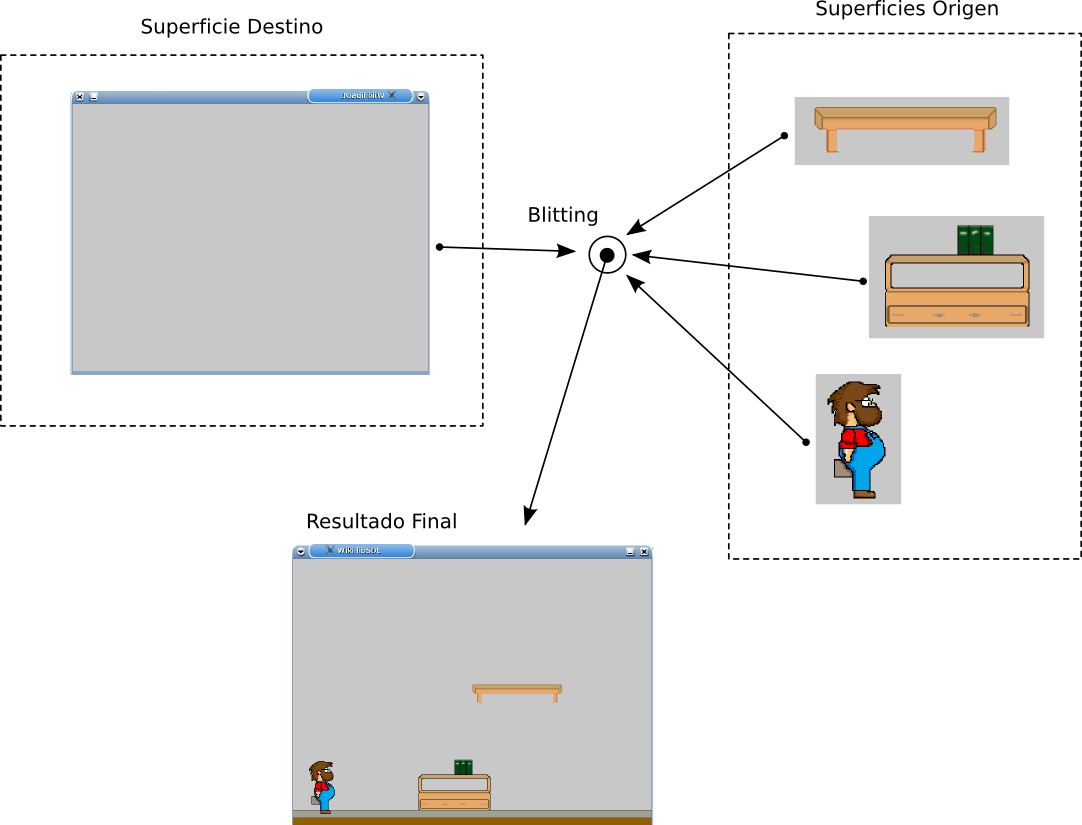
\includegraphics[scale=0.5]{img/Blitting.png}
	\end{center}
    
\end{frame}

\begin{frame}
    \frametitle{El Flipping y el doble buffer}
    
	\begin{block}{Doble buffer}
        \begin{itemize}
            \item Tenemos dos superficies: pantalla y auxiliar
            \item Hacemos blitting sobre la auxiliar
            \item Terminamos de componer la escena
            \item Intercambiamos pantalla y auxiliar
            \item Evitamos un horroroso parpadeo
        \end{itemize}            
    \end{block}
    
\end{frame}

\begin{frame}
    \frametitle{Flipping - Ejemplo}

    \begin{center}
		
\includegraphics[scale=2]{img/flipping.png}
	\end{center}
    
\end{frame}


\section{Implementación}
\begin{frame}
	\frametitle{Pong - Diagrama}
	
    \begin{center}
        Visión general del sistema
    \end{center}
	
    \begin{center}
		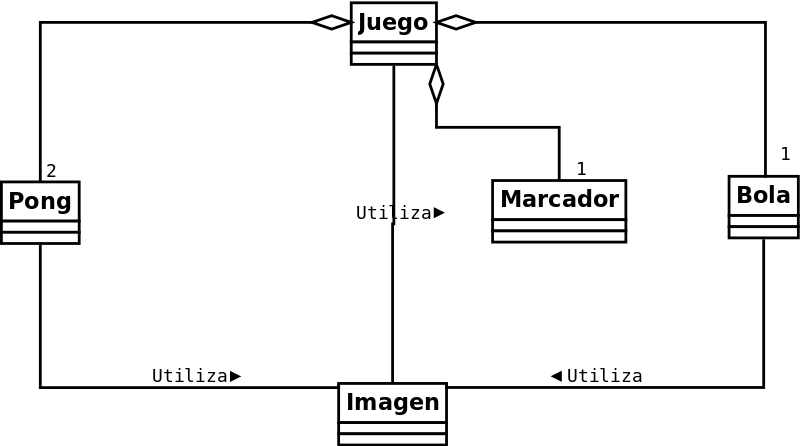
\includegraphics[scale=0.25]{img/modulos.png}
	\end{center}	

\end{frame}

\begin{frame}[fragile]
	\frametitle{Pong - Estructura del proyecto}
    
    \begin{columns}[c]
	\column{175pt}

\begin{verbatim}
|- pong
    |- makefile
    |- main.c
    |- motor
    |    |- fichero.c
    |    |- fichero.h
    |    |- (...)
    |
    |- multimedia
    |    |- imagen.png
    |    |- fuente.ttf
    |    |- (...)
\end{verbatim}
	
	\column{125pt}
	\begin{center}
		
\includegraphics[scale=0.4]{img/Binary-tree-256.png}
	\end{center}	
	
    \end{columns}

\end{frame}


\begin{frame}[fragile]
	\frametitle{En cada paso}
    
    \begin{columns}[c]
	\column{175pt}

	\begin{center}
	    Vamos a estructurar cada paso de la siguiente manera:
	\end{center}
	
	\begin{block}{En cada paso}
	    \begin{itemize}
		\item Objetivos del paso
		\item Algún concepto
		\item Funciones SDL necesarias
		\item Hora de currar
		\item Resultado
	    \end{itemize}
	\end{block}
	
	\column{125pt}
	\begin{center}
		
\includegraphics[scale=0.3]{img/1up.jpg}
	\end{center}	
	
    \end{columns}

\end{frame}

\begin{frame}
	\frametitle{Pong - Paso 1}
	
    \begin{columns}[c]
	\column{175pt}
	\begin{block}{Objetivos}
		\begin{itemize}
			\item Inicializar SDL
			\item Crear una ventana
			\item Esperar evento de salida
			\item Cerrar SDL
		\end{itemize}            
	\end{block}
    \column{125pt}
	\begin{center}
		
\includegraphics[scale=0.6]{img/checklist.jpg}
	\end{center}	
	
    \end{columns}

\end{frame}

\begin{frame}[fragile]
    \frametitle{Pong - Paso 1 - SDL\_Init}
	
\begin{verbatim}
int SDL_Init(Uint32 flags);
\end{verbatim}

    \begin{block}{SDL\_Init}
	Inicia SDL y los subsistemas que queramos
	
	\emph{Parámetros}:
	\begin{itemize}
	    \item Uint32 flags: susbistemas a inicializar. Se combinan con $||$
		\begin{itemize}
		    \item SDL\_INIT\_TIMER
		    \item SDL\_INIT\_AUDIO
		    \item SDL\_INIT\_VIDEO
		    \item SDL\_INIT\_CDROM
		    \item SDL\_INIT\_JOYSTICK
		    \item SDL\_INIT\_EVERYTHING
		\end{itemize}
	\end{itemize}
	
	\emph{Devuelve}: $0$ si tiene éxito, $-1$ en caso contrario

    \end{block}

\end{frame}

\begin{frame}[fragile]
    \frametitle{Pong - Paso 1 - SDL\_Quit}
	
\begin{verbatim}
void SDL_Quit(void);
\end{verbatim}

    \begin{block}{SDL\_Quit}
	Cierra SDL y todos sus subsistemas
    \end{block}

\end{frame}

\begin{frame}[fragile]
    \frametitle{Pong - Paso 1 - atexit}
	
\begin{verbatim}
int atexit(void (*function) (void));
\end{verbatim}

    \begin{block}{atexit}
	Llama a una función de tipo \emph{void funcion(void)} al terminar la ejecución
	
	\emph{Parámetros}:
	\begin{itemize}
	    \item void (*function) (void): puntero a una función que recibe y devuelve void.
	    
	    Ejemplo:
	    \begin{verbatim}
	    atexit(SDL_Quit);
	    \end{verbatim}
	\end{itemize}
	
	\emph{Devuelve}: $0$ si tiene éxito, distinto si falla
    \end{block}

\end{frame}

\begin{frame}[fragile]
    \frametitle{Pong - Paso 1 - SDL\_SetVideoMode}
	
\begin{verbatim}
SDL_Surface *SDL_SetVideoMode(int width, int height,
                              int bpp, Uint32 flags);
\end{verbatim}

    \begin{block}{SDL\_SetVideoMode}
	Crea la superficie principal (nuestra ventana)
	
	\emph{Parámetros}:
	\begin{itemize}
	    \item int width: ancho en píxeles
	    \item int height: alto en píxeles
	    \item int bpp: bits por píxel (profundidad)
	    \item Uint32 flags: opciones:
	    \begin{itemize}
		    \item SDL\_HWSURFACE
		    \item SDL\_DOUBLEBUF
	    \end{itemize}
	\end{itemize}
	
	\emph{Devuelve}: superficie principal o NULL si hay erores
    \end{block}

\end{frame}

\begin{frame}[fragile]
    \frametitle{Pong - Paso 1 - SDL\_WM\_SetCaption}
	
\begin{verbatim}
void SDL_WM_SetCaption(const char *title,
                       const char *icon);
\end{verbatim}

    \begin{block}{SDL\_WM\_SetCaption}
	Establece título e icono de la ventana
	
	\emph{Parámetros}:
	\begin{itemize}
	    \item const char *title: cadena con el título ("Pong")
	    \item const char *icon: cadena con la ruta del icono
	\end{itemize}
    \end{block}

\end{frame}

\begin{frame}[fragile]
    \frametitle{Pong - Paso 1 - SDL\_ShowCursor}
	
\begin{verbatim}
int SDL_ShowCursor(int toggle);
\end{verbatim}

    \begin{block}{SDL\_ShowCursor}
	Muestra u oculta el cursor en la ventana
	
	\emph{Parámetros}:
	\begin{itemize}
	    \item int toggle: SDL\_ENABLE, SDL\_DISABLE o SDL\_QUERY (consultar)
	\end{itemize}
	
	\emph{Devuelve}: estado del cursor (SDL\_ENABLE o SDL\_DISABLE)
    \end{block}

\end{frame}

\begin{frame}[fragile]
    \frametitle{Pong - Paso 1 - TTF\_Init}
	
\begin{verbatim}
int TTF_Init();
\end{verbatim}

    \begin{block}{TTF\_Init}
	Inicializa librería auxiliar para fuentes
	
	\emph{Devuelve}: $0$ si tiene éxito, $-1$ en caso contrario
    \end{block}

\end{frame}

\begin{frame}[fragile]
    \frametitle{Pong - Paso 1 - SDL\_GetKeyState}
	
\begin{verbatim}
Uint8 *SDL_GetKeyState(int *numkeys);
\end{verbatim}

    \begin{block}{SDL\_GetKeyState}
	Captura el estado del teclado completo
	
	\emph{Parámetros}:
	\begin{itemize}
	    \item int *numkeys: aquí se almacena el número de teclas (podemos pasarle NULL)
	\end{itemize}
	
	\emph{Devuelve}: vector con el teclado mapeado.	Ejemplo:
\begin{verbatim}
teclado = SDL_GetKeyState(NULL);
if(teclado[SDLK_UP])
    /* Hemos pulsado arriba */
\end{verbatim}
\end{block}

\end{frame}

\begin{frame}
	\frametitle{Pong - Paso 1}
	
    \begin{center}
        \textbf{¡Hora de currar!}
    \end{center}
	
    \begin{center}
		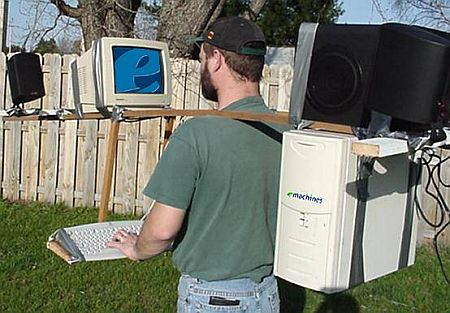
\includegraphics[scale=0.4]{img/currar-1.jpg}
    \end{center}	

\end{frame}

\begin{frame}
	\frametitle{Pong - Paso 1}
	
    \begin{center}
        \textbf{Resultado}
    \end{center}
	
    \begin{center}
		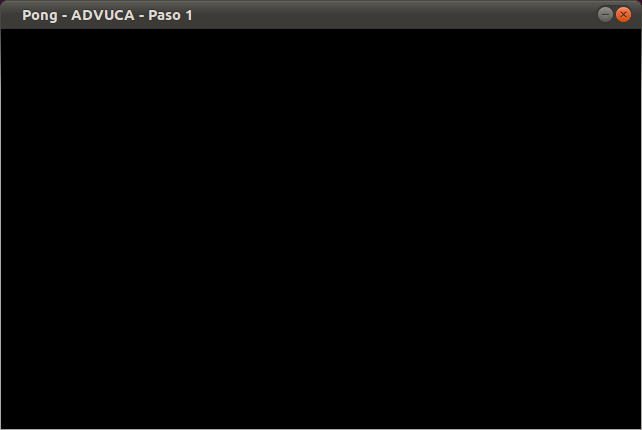
\includegraphics[scale=0.4]{img/pong-advuca-1.png}
    \end{center}	

\end{frame}

\begin{frame}
	\frametitle{Pong - Paso 2}
    \begin{columns}[c]
	\column{175pt}
	\begin{block}{Objetivos}
		\begin{itemize}
			\item Módulo de carga y dibujado de imágenes
			\item Cargar mesa de juego
		\end{itemize}            
	\end{block}

    \column{125pt}
	\begin{center}
		
\includegraphics[scale=0.6]{img/checklist.jpg}
	\end{center}	
	
    \end{columns}
\end{frame}

\begin{frame}[fragile]
    \frametitle{Pong - Paso 2 - IMG\_Load}
	
\begin{verbatim}
SDL_Surface *IMG_Load(const char *file);
\end{verbatim}

    \begin{block}{IMG\_Load}
	Carga una imagen
	
	\emph{Parámetros}:
	\begin{itemize}
	    \item const char *file: ruta de la imagen a cargar
	\end{itemize}
	
	\emph{Devuelve}: superficie con la imagen cargada, NULL si falla
    \end{block}

\end{frame}

\begin{frame}[fragile]
    \frametitle{Pong - Paso 2 - SDL\_DisplayFormatAlpha}
	
\begin{verbatim}
SDL_Surface *SDL_DisplayFormatAlpha(SDL_Surface *surface);
\end{verbatim}

    \begin{block}{SDL\_DisplayFormatAlpha}
	Adapta una superficie con transparencia al formato de la pantalla
	
	\emph{Parámetros}:
	\begin{itemize}
	    \item SDL\_Surface *surface: superficie a adaptar
	\end{itemize}
	
	\emph{Devuelve}: superficie con la imagen adaptada, NULL si falla
    \end{block}

\end{frame}

\begin{frame}[fragile]
    \frametitle{Pong - Paso 2 - SDL\_FreeSurface}
	
\begin{verbatim}
void SDL_FreeSurface(SDL_Surface *surface);
\end{verbatim}

    \begin{block}{SDL\_FreeSurface}
	Libera la memoria ocupada por la superficie
	
	\emph{Parámetros}:
	\begin{itemize}
	    \item SDL\_Surface *surface: superficie a eliminar
	\end{itemize}
    \end{block}
    
    \begin{center}
    \textbf{¡No se usa \emph{free(surface);} !}
    \end{center}

\end{frame}

\begin{frame}[fragile]
    \frametitle{Pong - Paso 2 - SDL\_BlitSurface}
	
\begin{verbatim}
int SDL_BlitSurface(SDL_Surface *src, SDL_Rect *srcrect,
                    SDL_Surface *dst, SDL_Rect *dstrect);
\end{verbatim}

    \begin{block}{SDL\_BlitSurface}
	Pega la superficie origen en la superficie destino
	
	\emph{Parámetros}:
	\begin{itemize}
	    \item SDL\_Surface *src: superficie origen
	    \item SDL\_Rect *srcrect: recuadro de la imagen origen a copiar
	    \item SDL\_Surface *dst: superficie destino
	    \item SDL\_Rect *drcrect: recuadro de la imagen destino a ocupar
	\end{itemize}
	
	\emph{Devuelve}: $0$ si todo va bien, $-1$ si falla.
    \end{block}

\end{frame}

\begin{frame}[fragile]
    \frametitle{Pong - Paso 2 - SDL\_Flip}
	
\begin{verbatim}
int SDL_Flip(SDL_Surface *screen);
\end{verbatim}

    \begin{block}{SDL\_Flip}
	Intercambia el buffer temporal con la ventana (muestra nuestro \emph{collage})
	
	\emph{Parámetros}:
	\begin{itemize}
	    \item SDL\_Surface *screen: superficie principal que representa a la ventana
	\end{itemize}
	
	\emph{Devuelve}: $0$ si todo va bien, $-1$ si falla.
    \end{block}

\end{frame}

\begin{frame}
	\frametitle{Pong - Paso 2}
	
    \begin{center}
        \textbf{¡Hora de currar!}
    \end{center}
	
    \begin{center}
		
\includegraphics[scale=0.4]{img/currar-2.jpg}
	\end{center}	

\end{frame}

\begin{frame}
	\frametitle{Pong - Paso 2}
	
    \begin{center}
        \textbf{Resultado}
    \end{center}
	
    \begin{center}
		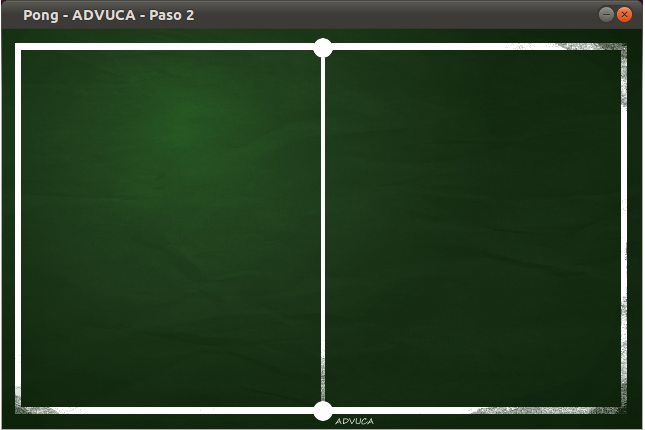
\includegraphics[scale=0.4]{img/pong-advuca-2.png}
	\end{center}	

\end{frame}

\begin{frame}
	\frametitle{Pong - Paso 3}
    \begin{columns}[c]
	\column{175pt}
	\begin{block}{Objetivos}
		\begin{itemize}
			\item Módulo para las palas
			\item Control de la pala del jugador 1
			\item Control de FPS
		\end{itemize}            
	\end{block}

    \column{125pt}
	\begin{center}
		
\includegraphics[scale=0.6]{img/checklist.jpg}
	\end{center}	
	
    \end{columns}
\end{frame}

\begin{frame}[fragile]
    \frametitle{Pong - Paso 3 - SDL\_GetTicks}
	
\begin{verbatim}
Uint32 SDL_GetTicks(void);
\end{verbatim}

    \begin{block}{SDL\_GetTicks}
	\emph{Devuelve}: milisegundos desde que inicializamos SDL
    \end{block}
    
    Si llamamos a \emph{SDL\_GetTicks} en cada frame, podremos conocer
    el tiempo que pasa entre frames.
    
\begin{verbatim}
Uint32 t0 = SDL_GetTicks();

while(!salir) {
    t1 = SDL_GetTicks();
    printf("Tiempo entre frames %d\n", t1 - t0);
    t0 = t1;
}
\end{verbatim}

\end{frame}

\begin{frame}[fragile]
    \frametitle{Pong - Paso 3 - SDL\_Delay}
	
\begin{verbatim}
void SDL_Delay(Uint32 ms);
\end{verbatim}

    \begin{block}{SDL\_Delay}
	Inserta un retardo en nuestra aplicación
	
	\emph{Parámetros}:
	\begin{itemize}
	    \item Uint32 ms: entero indicando los milisegundos que esperaremos
	\end{itemize}
	
	Lo utilizamos para controlar el \emph{framerate}
    \end{block}
    
    Tiempo de espera:
\begin{verbatim}
if((t1 - t0) < (1000 / FPS))
     SDL_Delay((1000 / FPS) - (t1 - t0));
\end{verbatim}

\end{frame}


\begin{frame}
	\frametitle{Pong - Paso 3}
	
    \begin{center}
        \textbf{¡Hora de currar!}
    \end{center}
	
    \begin{center}
		
\includegraphics[scale=0.4]{img/currar-6.png}
	\end{center}	

\end{frame}

\begin{frame}
	\frametitle{Pong - Paso 3}
	
    \begin{center}
        \textbf{Resultado}
    \end{center}
	
    \begin{center}
		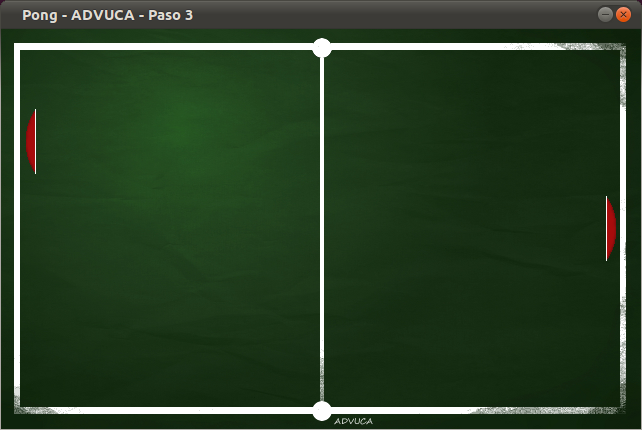
\includegraphics[scale=0.4]{img/pong-advuca-3.png}
	\end{center}	

\end{frame}

\begin{frame}
	\frametitle{Pong - Paso 4}
    \begin{columns}[c]
	\column{175pt}
	\begin{block}{Objetivos}
		\begin{itemize}
			\item Módulo de la pelota
			\item Rebote básico de la pelota en bordes
			\item La pelota atraviesa las palas (por ahora)
		\end{itemize}            
	\end{block}
    \column{125pt}
	\begin{center}
		
\includegraphics[scale=0.6]{img/checklist.jpg}
	\end{center}	
	
    \end{columns}
\end{frame}

\begin{frame}
	\frametitle{Pong - Paso 4}
	
    \begin{center}
        \textbf{¡Hora de currar!}
    \end{center}
	
    \begin{center}
		
\includegraphics[scale=0.4]{img/currar-4.jpg}
	\end{center}	

\end{frame}

\begin{frame}
	\frametitle{Pong - Paso 4}
	
    \begin{center}
        \textbf{Resultado}
    \end{center}
	
    \begin{center}
		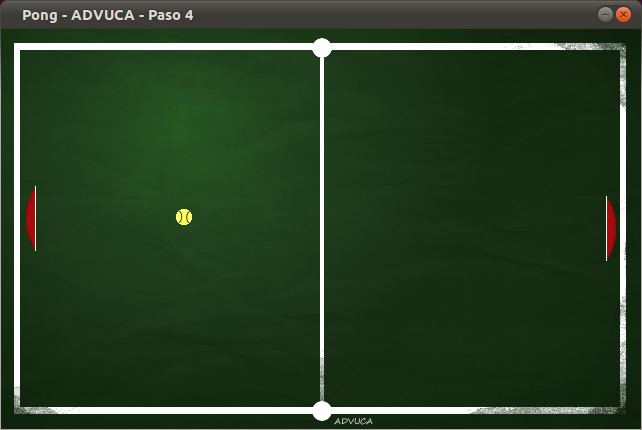
\includegraphics[scale=0.4]{img/pong-advuca-4.png}
	\end{center}	

\end{frame}

\begin{frame}
	\frametitle{Pong - Paso 5}
    \begin{columns}[c]
	\column{175pt}
	\begin{block}{Objetivos}
		\begin{itemize}
			\item Colisión con las palas
			\item Inteligencia artificial
			\item La IA sigue a la pelota en el eje Y
		\end{itemize}            
	\end{block}
    
    \column{125pt}
	\begin{center}
		
\includegraphics[scale=0.6]{img/checklist.jpg}
	\end{center}	
	
    \end{columns}
\end{frame}

\begin{frame}
	\frametitle{Pong - Paso 5}
	
    \begin{center}
        \textbf{¡Hora de currar!}
    \end{center}
	
    \begin{center}
		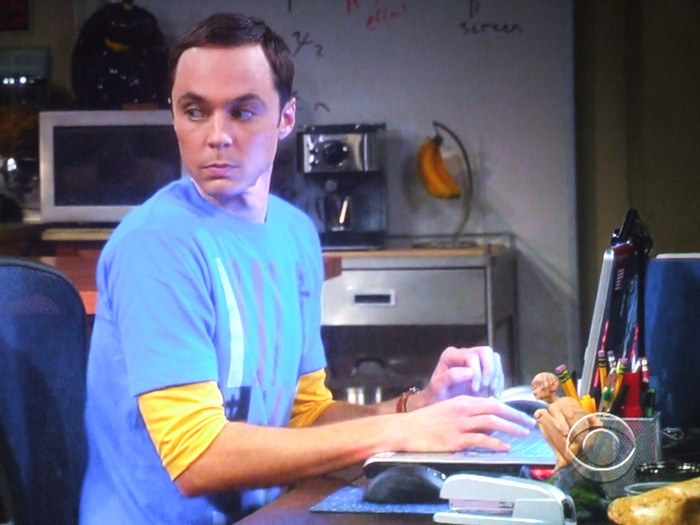
\includegraphics[scale=0.3]{img/currar-5.jpg}
	\end{center}	

\end{frame}

\begin{frame}
	\frametitle{Pong - Paso 5}
	
    \begin{center}
        \textbf{Resultado}
    \end{center}
	
    \begin{center}
		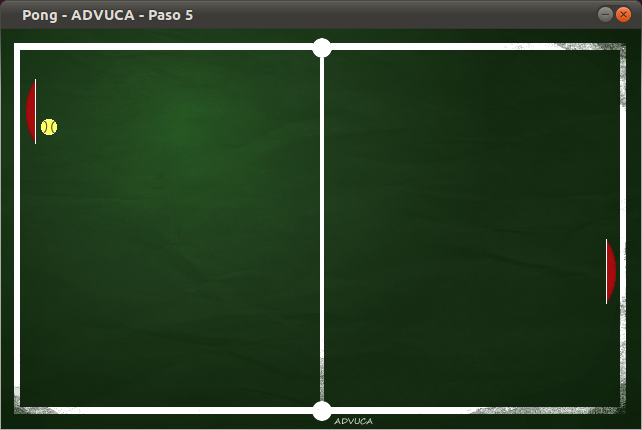
\includegraphics[scale=0.4]{img/pong-advuca-5.png}
	\end{center}	

\end{frame}

\begin{frame}
	\frametitle{Pong - Paso 6}
    \begin{columns}[c]
	\column{175pt}
	\begin{block}{Objetivos}
		\begin{itemize}
			\item Creación del módulo marcador
			\item Si el jugador golpea la bola, suma un punto
			\item Se mantiene el récord de golpeos
			\item El marcador se reinicia si el jugador falla
		\end{itemize}            
	\end{block}
	
    \column{125pt}
	\begin{center}
		
\includegraphics[scale=0.6]{img/checklist.jpg}
	\end{center}	
	
    \end{columns}
\end{frame}

\begin{frame}[fragile]
    \frametitle{Pong - Paso 6 - TTF\_OpenFont}
	
\begin{verbatim}
TTF_Font *TTF_OpenFont(const char *file,
                       int ptsize);
\end{verbatim}

    \begin{block}{TTF\_OpenFont}
	Carga una fuente ttf en memoria
	
	\emph{Parámetros}:
	\begin{itemize}
	    \item const char *file: ruta del fichero con la fuente
	    \item int ptsize: tamaño en puntos de la fuente
	\end{itemize}
	
	\emph{Devuelve}: fuente lista para ser utilizada, NULL si hay errores

    \end{block}

\end{frame}

\begin{frame}[fragile]
    \frametitle{Pong - Paso 6 - TTF\_CloseFont}
	
\begin{verbatim}
void TTF_CloseFont(TTF_Font *font);
\end{verbatim}

    \begin{block}{TTF\_CloseFont}
	Libera la memoria ocupada por la fuente
	
	\emph{Parámetros}:
	\begin{itemize}
	    \item TTF\_Font *font: fuente a eliminar
	\end{itemize}

    \end{block}

\end{frame}

\begin{frame}[fragile]
    \frametitle{Pong - Paso 6 - TTF\_RenderUTF8\_Blended}
	
\begin{verbatim}
SDL_Surface *TTF_RenderUTF8_Solid(TTF_Font *font,
                                  const char *text,
                                  SDL_Color fg);
\end{verbatim}

    \begin{block}{TTF\_RenderUTF8\_Solid}
	Renderiza texto en una superficie SDL
	
	\emph{Parámetros}:
	\begin{itemize}
	    \item TTF\_Font *font: fuente a utilizar en el renderizado
	    \item const char *text: cadena a renderizar
	    \item SDL\_Color fg: color del texto
	\end{itemize}
	
	\emph{Devuelve}: superficie SDL

    \end{block}
    
    Para adaptar la superficie deberemos llamar a \emph{SDL\_DisplayFormatAlpha}
    antes de hacer \emph{SDL\_BlitSurface}

\end{frame}

\begin{frame}
	\frametitle{Pong - Paso 6}
	
    \begin{center}
        \textbf{¡Hora de currar!}
    \end{center}
	
    \begin{center}
		
\includegraphics[scale=0.7]{img/currar-3.jpg}
	\end{center}	

\end{frame}

\begin{frame}
	\frametitle{Pong - Paso 6}
	
    \begin{center}
        \textbf{Resultado}
    \end{center}
	
    \begin{center}
		\includegraphics[scale=0.4]{img/pong-advuca-6.png}
	\end{center}	

\end{frame}


\section{Ampliación}
\begin{frame}
	\frametitle{Añadidos del Pong}
	
    
	\begin{columns}[c]
		\column{200pt}
		
	\begin{block}{Lo que se puede mejorar}
            \begin{itemize}
                \item Mejores gráficos (¡trabaja siempre con artistas!)
                \item Inteligencia Artificial torpe
                \item Efectos de sonido (rebote, victoria, derrota)
                \item Guardar la puntuación en un fichero
		\item Mejora del rendimiento
            \end{itemize}            
        \end{block}        
		
        \column{100pt}
		\begin{center}
			\includegraphics[scale=0.32]{img/expand.jpg}
		\end{center}
        
	\end{columns} 

\end{frame}


\begin{frame}
	\frametitle{Cambiamos a PyGame}
	
	      
	Nuestro \emph{querido} amigo Jose nos enseñará su Pong (powered by PyGame)
	
	\begin{center}
	    \includegraphics[scale=0.32]{img/pygame.png}
	\end{center}

\end{frame}



\section{Más allá}

%	======= 1) NOW WHAT? =======

\begin{frame}
	\frametitle{Muy bien pero...¿Cómo sigo?}
	
	\begin{center}
		\includegraphics[scale=0.40]{img/nowwhat.jpg}
	\end{center}

\end{frame}

%	======= 2) REQUISITOS =======

\begin{frame}
	\frametitle{¿Qué necesito?}
	
	Como has podido ver desarrollar un videojuego no es tarea fácil, requiere de un proceso de constante aprendizaje, investigación, dedicación y mucha ayuda.
		
	\begin{block}{Recomendaciones}
		\begin{itemize}
			\item Motivación: Hay que dedicarle mucho tiempo.
			\item Curiosidad: Interés por aprender cosas nuevas y mejorar lo que ya sabes.
			\item Saber Inglés: Gran cantidad de los recursos de calidad están en inglés.
			\item Contactos: Trabajo artístico, publicitario, sonido, beta testers...
			\item Comunidad: Lugar de referencia para consultar, compartir, etc.
		\end{itemize}
	\end{block}

\end{frame}

%	======= 3) LENGUAJES =======

\begin{frame}
	\frametitle{Lenguajes Alto Nivel}
	
	Según los conocimientos que tengas, así como los propósitos y metas del juego a desarrollar es importante elegir bien el lenguaje de programación.
		
	\begin{block}{Recomendaciones}
		\begin{itemize}
			\item C/C++/C\#
			\item Python
			\item Java
			\item Lua
			\item Lisp
			\item Ruby
		\end{itemize}
	\end{block}

\end{frame}

%	======= 4) LIBRERÍAS 2D =======

\begin{frame}
	\frametitle{Librerías 2D}
		
	La mejor forma de adentrarse en el desarrollo de videojuegos.

	\begin{block}{Algunos ejemplos destacados}
		\begin{itemize}
			\item Gosu
			\item SDL
			\item Allegro
			\item Pygame
			\item ClanLib
		\end{itemize}
	\end{block}

\end{frame}

%	======= 5) LIBRERÍAS 3D =======

\begin{frame}
	\frametitle{Librerías 3D}
	\begin{columns}[c]
		\column{150pt}
			El salto de calidad...
		\column{150pt}
			\begin{center}
				\includegraphics[scale=0.05]{img/2dto3d.jpg}
			\end{center}
	\end{columns}
	\begin{block}{Algunos ejemplos destacados}
		\begin{itemize}
			\item Ogre
			\item IrrLicht
			\item Crystal Space
			\item Panda
		\end{itemize}
	\end{block}

	\begin{center}
		\includegraphics[scale=0.45]{img/logos.png}
	\end{center}

\end{frame}

%	======= 6) LIBRERÍAS AUXILIARES =======

\begin{frame}
	\frametitle{Otras Librerías y Herramientas}
		
	En muchas ocasiones es necesario apoyarse en otras librerías externas o herramientas que desarrollarán funciones auxiliares.
	\newline
	\begin{block}{Algunos ejemplos destacados}
		\begin{itemize}
			\item Física: ODE, BULLET.
			\item Gestión de Entrada: OIS.
			\item Diseño Artístico: Gimp, Blender.
		\end{itemize}
	\end{block}

\end{frame}

%	======= 7) RECURSOS BIBLIOGRÁFICOS =======

\begin{frame}
	\frametitle{La biblioteca}
	
	\begin{center}
		\includegraphics[scale=0.50]{img/biblio.jpg}
	\end{center}

\end{frame}

%	======= 8) TRABAJO EN EQUIPO =======

\begin{frame}
	\frametitle{Trabajo en Equipo}
	
	\begin{center}
		\includegraphics[scale=0.70]{img/equipo.jpg}
	\end{center}

\end{frame}

%	======= 9) ADVUCA, TU AMIGO FIEL =======

\begin{frame}
	\frametitle{ADVUCA}
		
	Desde la ADVUCA nos comprometemos a ofrecer ayuda para fomentar desarrollo de proyectos e incentivar el aprendizaje a través de los videojuegos.

	\begin{block}{Algunos ejemplos destacados}
		\begin{itemize}
			\item Formación de grupos de trabajo(juegos, manuales, etc).
			\item Difusión.
			\item Consultas.
		\end{itemize}
	\end{block}

	\begin{center}
		\includegraphics[scale=0.50]{img/micro.png}
	\end{center}

\end{frame}

%	======= 10) MUNDO LABORAL =======

\begin{frame}
	\frametitle{El Exterior...}
		
	Después de la UCA, empieza lo bueno...

	\begin{columns}[c]
		\column{150pt}
			\begin{block}{Algunas posibilidades}
				\begin{itemize}
					\item Masters.
					\item Desarrolladoras de Videojuegos.
					\item Centros Multimedia.
				\end{itemize}
			\end{block}
		\column{150pt}
			\begin{center}
				\includegraphics[scale=0.15]{img/exterior.jpg}
			\end{center}
	\end{columns}
\end{frame}




\section{Opiniones}
\begin{frame}
	\frametitle{¡Gracias!}
	
	\begin{center}
    \huge{¡Muchas gracias por venir!}
    \end{center}
		
    \begin{center}
        \emph{No lancen los tomates todavía}
    \end{center}
    
	\begin{columns}[c]
	\column{200pt}	
	
	\begin{block}{Nos interesa vuestra opinión}
        \begin{itemize}
            \item ¿Opinión del taller?
            \item Cosas para mejorar
            \item Temas que interesa tratar
        \end{itemize}
    \end{block}
	
	\column{100pt}
	\begin{center}
	    \includegraphics[scale=0.3]{img/thumbs-up.jpg}
	\end{center}   
    
    \end{columns}  
	
\end{frame}


\end{document}
